\documentclass[10pt]{beamer}
\usetheme[
%%% options passed to the outer theme
%    hidetitle,           % hide the (short) title in the sidebar
%    hideauthor,          % hide the (short) author in the sidebar
%    hideinstitute,       % hide the (short) institute in the bottom of the sidebar
%    shownavsym,          % show the navigation symbols
%    width=2cm,           % width of the sidebar (default is 2 cm)
%    hideothersubsections,% hide all subsections but the subsections in the current section
%    hideallsubsections,  % hide all subsections
    left               % right of left position of sidebar (default is right)
%%% options passed to the color theme
%    lightheaderbg,       % use a light header background
  ]{AAUsidebar}

% If you want to change the colors of the various elements in the theme, edit and uncomment the following lines
% Change the bar and sidebar colors:
%\setbeamercolor{AAUsidebar}{fg=red!20,bg=red}
%\setbeamercolor{sidebar}{bg=red!20}
% Change the color of the structural elements:
%\setbeamercolor{structure}{fg=red}
% Change the frame title text color:
%\setbeamercolor{frametitle}{fg=blue}
% Change the normal text color background:
%\setbeamercolor{normal text}{bg=gray!10}
% ... and you can of course change a lot more - see the beamer user manual.


\usepackage[utf8]{inputenc}
\usepackage[english]{babel}
\usepackage[T1]{fontenc}
% Or whatever. Note that the encoding and the font should match. If T1
% does not look nice, try deleting the line with the fontenc.
\usepackage{helvet}

\usepackage[lined,boxed,commentsnumbered,linesnumbered]{algorithm2e}
\setlength{\algomargin}{2em}

\usetikzlibrary{arrows,automata,positioning}

\usepackage{amsmath}

% colored hyperlinks
\newcommand{\chref}[2]{%
  \href{#1}{{\usebeamercolor[bg]{AAUsidebar}#2}}%
}

\title[CTIF]% optional, use only with long paper titles
{C Timed Information Flow}

%\subtitle{v.\ 1.4.0}  % could also be a conference name

\date{June 8, 2016}

\author[Christensen \& Larsen] % optional, use only with lots of authors
{
  Mikael Elkiær Christensen, \href{mailto:michri11@student.aau.dk}{{\tt michri11@student.aau.dk}}\\
  Mikkel Sandø Larsen, \href{mailto:milars11@student.aau.dk}{{\tt milars11@student.aau.dk}}
}
% - Give the names in the same order as they appear in the paper.
% - Use the \inst{?} command only if the authors have different
%   affiliation. See the beamer manual for an example

\institute[
%  {\includegraphics[scale=0.2]{aau_segl}}\\ %insert a company, department or university logo
  Dept.\ of Computer Science\\
  Aalborg University\\
  Denmark
] % optional - is placed in the bottom of the sidebar on every slide
{% is placed on the title page
  Department of Computer Science\\
  Aalborg University\\
  Denmark

  %there must be an empty line above this line - otherwise some unwanted space is added between the university and the country (I do not know why;( )
}


% specify a logo on the titlepage (you can specify additional logos an include them in
% institute command below
\pgfdeclareimage[height=1.5cm]{titlepagelogo}{AAUgraphics/aau_logo_new} % placed on the title page
%\pgfdeclareimage[height=1.5cm]{titlepagelogo2}{graphics/aau_logo_new} % placed on the title page
\titlegraphic{% is placed on the bottom of the title page
  \pgfuseimage{titlepagelogo}
%  \hspace{1cm}\pgfuseimage{titlepagelogo2}
}


\begin{document}
% the titlepage
{\aauwavesbg%
\begin{frame}[plain,noframenumbering] % the plain option removes the sidebar and header from the title page
  \titlepage
\end{frame}}
%%%%%%%%%%%%%%%%

% TOC
\begin{frame}{Agenda}{}
\tableofcontents
\end{frame}
%%%%%%%%%%%%%%%%

%%%%%%%%%%%%%%
% INTRODUCTION
%%%%%%%%%%%%%%
\section{Introduction}

\begin{frame}
  \frametitle{Embedded Devices / IoT}
  \let\thefootnote\relax\footnotetext{\tiny{\url{https://www-ssl.intel.com/content/www/us/en/internet-of-things/infographics/guide-to-iot.html}}}
  Estimated number of devices:
  \begin{itemize}
    \item 2006: 2 billion
    \item 2015: 15 billion
    \item 2020: 200 billion
  \end{itemize}
  \vspace{1em}
  Usage:
  \begin{itemize}
    \item 40.2 \% Business/manufacturing
    \item 30.3 \% Health care
    \item 8.3 \% Retail
    \item 7.7 \% Security
  \end{itemize}
\end{frame}

\begin{frame}
  \frametitle{Programmer's Perspective}

  Extension to C:
  \begin{itemize}
    \item Simple syntax
    \item Minimal intrusiveness
    \item Compiler errors
    \item (Visual aids)
  \end{itemize}
\end{frame}

\begin{frame}
  \frametitle{Arduino and Raspberry}
  Estimated sold units:
  \begin{itemize}
    \item Arduino -- 1.5 million (2013)\footnote{\tiny\url{http://medea.mah.se/2013/04/arduino-faq/}}
    \item Raspberry Pi -- 3 million (2014)\footnote{\tiny\url{https://www.raspberrypi.org/blog/raspberry-pi-at-buckingham-palace-3-million-sold/}}
  \end{itemize}
  \vspace{1em}
  Implications:
  \begin{itemize}
    \item More exposed devices
    \item More amateur implementations
  \end{itemize}
\end{frame}

%%%%%%%%%%%%%%%%%%%%%%%%%%%
% DECENTRALIZED LABEL MODEL
%%%%%%%%%%%%%%%%%%%%%%%%%%%
\section[DLM]{Decentralized Label Model}

\subsection{Overview}
\begin{frame}
  \frametitle{Label policies}
  \centering

  \newcommand{\mathvspace}{\\[2em]}
    \[ L_1 = \{ o_1 \rightarrow r_1, r_2 \} \quad L_2 = \{ o_1 \rightarrow r_1 ; \; o_2 \rightarrow r_1 \} \]
    \[ L_1 \sqcup L_2  = \{ o_1 \rightarrow r_1 ; \; o_2 \rightarrow r_1 \} \]
    \[ L_1 \sqcap L_2  = \{ o_1 \rightarrow r_1, r_2 \} \]
    \[ L_2 \sqsubseteq L_1 \land L_1 \not\sqsubseteq L_2 \]
\end{frame}

\begin{frame}
  \frametitle{Abstract lattice}
  \begin{center}
    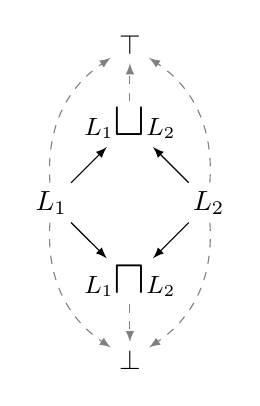
\begin{tikzpicture}[inner sep=1mm, >=latex]
      \node (l1) at (-1,0) {$L_1$};
      \node (l2) at (1,0) {$L_2$};

      \node (meet) at (0,-1) {\small $L_1$ {\LARGE $\! \sqcap \!$} $L_2$};
      \node (bot) at (0,-2) {$\bot$};

      \node (join) at (0,1) {\small $L_1$ {\LARGE $\! \sqcup \!$} $L_2$};
      \node (top) at (0,2) {$\top$};

      \draw[->] (l1) edge (join);
      \draw[->] (l2) edge (join);
      \draw[->] (l1) edge (meet);
      \draw[->] (l2) edge (meet);

      \draw[->, dashed, gray] (l1) edge [bend left] (top);
      \draw[->, dashed, gray] (join) edge (top);
      \draw[->, dashed, gray] (l2) edge [bend right] (top);

      \draw[->, dashed, gray] (l1) edge [bend right] (bot);
      \draw[->, dashed, gray] (meet) edge (bot);
      \draw[->, dashed, gray] (l2) edge [bend left] (bot);
    \end{tikzpicture}
  \end{center}
\end{frame}

\begin{frame}
  \frametitle{Example lattice}
  \scalebox{0.5}{\newcommand{\es}{\emptyset}
\newcommand{\pol}[2]{$\{ a \rightarrow #1; \; b \rightarrow #2 \}$}
\begin{tikzpicture}[->,>=stealth',shorten >=1pt,auto,node distance=3cm, semithick]
	\node (ao-bo) {\pol{\es}{\es}};

	\node (ab-bo) [below left of=ao-bo] {\pol{b}{\es}};
	\node (aa-bo) [left of=ab-bo] {\pol{a}{\es}};
	\node (ao-bb) [below right of=ao-bo] {\pol{\es}{b}};
	\node (ao-ba) [right of=ao-bb] {\pol{\es}{a}};

	\node (aa-bb) [below of=ab-bo] {\pol{a}{b}};
	\node (ab-ba) [below of=ao-bb] {\pol{b}{a}};
	\node (aa-ba) [left of=aa-bb] {\pol{a}{a}};
	\node (ao-bab) [left of=aa-ba] {\pol{\es}{a, b}};
	\node (ab-bb) [right of=ab-ba] {\pol{b}{b}};
	\node (aab-bo) [right of=ab-bb] {\pol{a, b}{\es}};

	\node (ab-bab) [below of=aa-bb] {\pol{b}{a, b}};
	\node (aab-ba) [below of=ab-ba] {\pol{a, b}{a}};
	\node (aab-bb) [below of=ab-bb] {\pol{a, b}{b}};
	\node (aa-bab) [below of=aa-ba] {\pol{a}{a, b}};
	
	\node (aab-bab) [below=10cm of ao-bo] {\pol{a, b}{a, b} $= \bot $};

	\path 	(aa-bab) edge (aab-bab)
				(ab-bab) edge (aab-bab)
				(aab-ba) edge (aab-bab)
				(aab-bb) edge (aab-bab);
	
\end{tikzpicture}
}
\end{frame}

\begin{frame}
  \frametitle{Constraint checking}

  Label types:
  \begin{itemize}
    \item Policy
    \item Variable
    \item Constant
    \item Composite labels (join/meet)
    \item Upper/lower bound
  \end{itemize}
  \vspace{1em}
  Output channel constraints:
  \begin{itemize}
    \item No simple check of reader sets
    \item Constraint for each argument, enabling inferrence
  \end{itemize}
\end{frame}

\subsection{Scope}
\begin{frame}
  \frametitle{Static \& Runtime}

  \begin{itemize}
    \item Principal hierarchy
    \item Label as first-class citizen
    \item Function call authority
    \item Run-time label checking
  \end{itemize}
\end{frame}

\begin{frame}
  \frametitle{Integrity}

\end{frame}

%%%%%%%%%%
% THE TOOL
%%%%%%%%%%
\section{The CTIF Tool}

\subsection{Process}
\begin{frame}
  \frametitle{Process}
  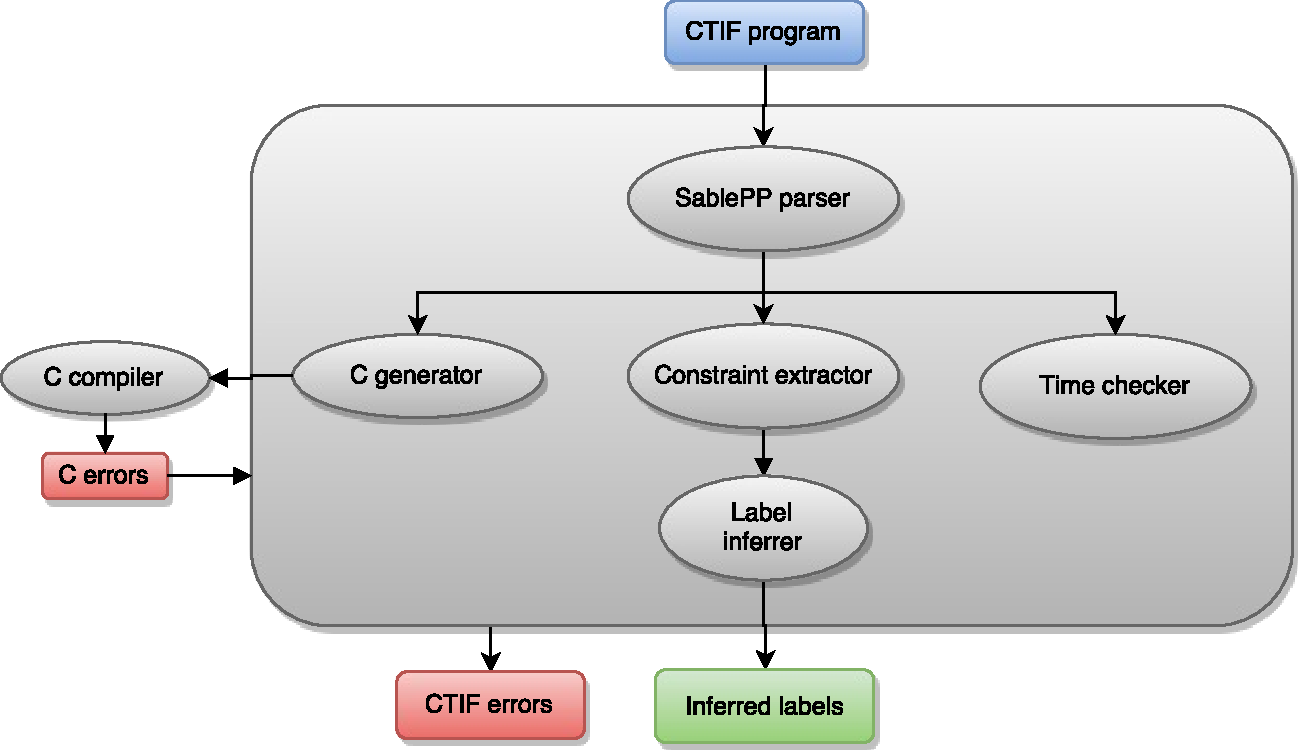
\includegraphics[width=\textwidth]{figures/thetool.pdf}
\end{frame}

\subsection{Demonstration}
\begin{frame}
  \frametitle{Demonstration}
  Demonstration!
\end{frame}

%%%%%%%%%%%
% INFERENCE
%%%%%%%%%%%
\section{Inference}

\subsection{Algorithm}
\begin{frame}
  \frametitle{Algorithm}
  \centering

  \scalebox{.9}{
  % !TEX root = ../master.tex
\begin{algorithm}[h]
\SetAlgoNoEnd
CHECK\_LABELS(p)\\
Function parameters without a label will get a constant label named after the parameter\\
Slots without a label will get a variable label named after the slot, with current upper bound set to $\top$\\
Conditional blocks will get a variable label named $L_i$, for blocks $0, 1, \dots, i$, where $L$ is the type of block\\
Declassifications will get variable labels named $D_{s_j}$ for declassifications $0, 1, \dots, j$, where $\underline{s}$ is the declassified slot\\
Let $Q$ be all constraints for program $p$, created as such:\\
For each assignment, the constraint is $\underline{block} \sqcup \underline{expr} \sqsubseteq \underline{slot}$\\
For each return statement, the constraint is $\underline{expr} \sqsubseteq returnLabel$\\
For each block $i$, the constraint is $\underline{block} \sqcup \underline{cond} \sqsubseteq \underline{L_i}$\\
For each declassification $j$, the constraint is $\underline{slot} \sqsubseteq \underline{L_{d_j}} \sqcup (\forall p \in authority \longrightarrow \{ p \rightarrow \emptyset\})$\\
\ForEach {$c \in Q$}
{
  \If {left($c$) is variable}
  {
    upper($c$) = $\top$
  }
  \Else
  {
    upper($c$) = left($c$)
  }
}
\While {$\exists c \in Q | upper(c) \sqsubseteq right(c)$}
{
  pick $c \in Q | upper(c) \sqsubseteq right(c)$\\
  \If {left($c$) is not variable}
  {
    $ERROR$
  }
  let upper($c$) = upper($c$) $\sqcup$ right($c$)
}
\end{algorithm}

  }
\end{frame}

\subsection{Polyvariance function evaluation}
\begin{frame}
  \frametitle{Polyvariance function evaluation}

\end{frame}

%%%%%%%%%%%%%%%
% TIME POLICIES
%%%%%%%%%%%%%%%
\section{Time Policies}

\subsection{Examples}
\begin{frame}
  \frametitle{Bill calculator}
  \centering

  \scalebox{1}{\newcommand{\ccc}{\texttt{get\_users}}
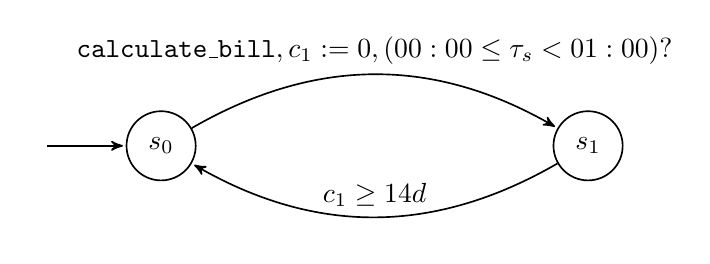
\begin{tikzpicture}[->,>=stealth',shorten >=1pt,auto,node distance=7cm, semithick]
	\node(start) {};
	\node[state] (S0) [right=0cm and 1cm of start]{$s_0$};
	\node[state] (S1) [right of=start] {$s_1$};

	\path[every node/.style={sloped,anchor=south,auto=false}]
	(start) edge node {} (S0)
	(S0) edge [bend left] node {$\texttt{calculate\_bill}, c_1 := 0, (00:00 \leq \tau_s < 01:00)?$} (S1)
	(S1) edge [bend left] node {$c_1 \geq 14d$} (S0);
\end{tikzpicture}
}
\end{frame}

\begin{frame}
  \frametitle{Password checker}
  \centering

  \scalebox{0.4}{\newcommand{\ccc}{\texttt{get\_users}}
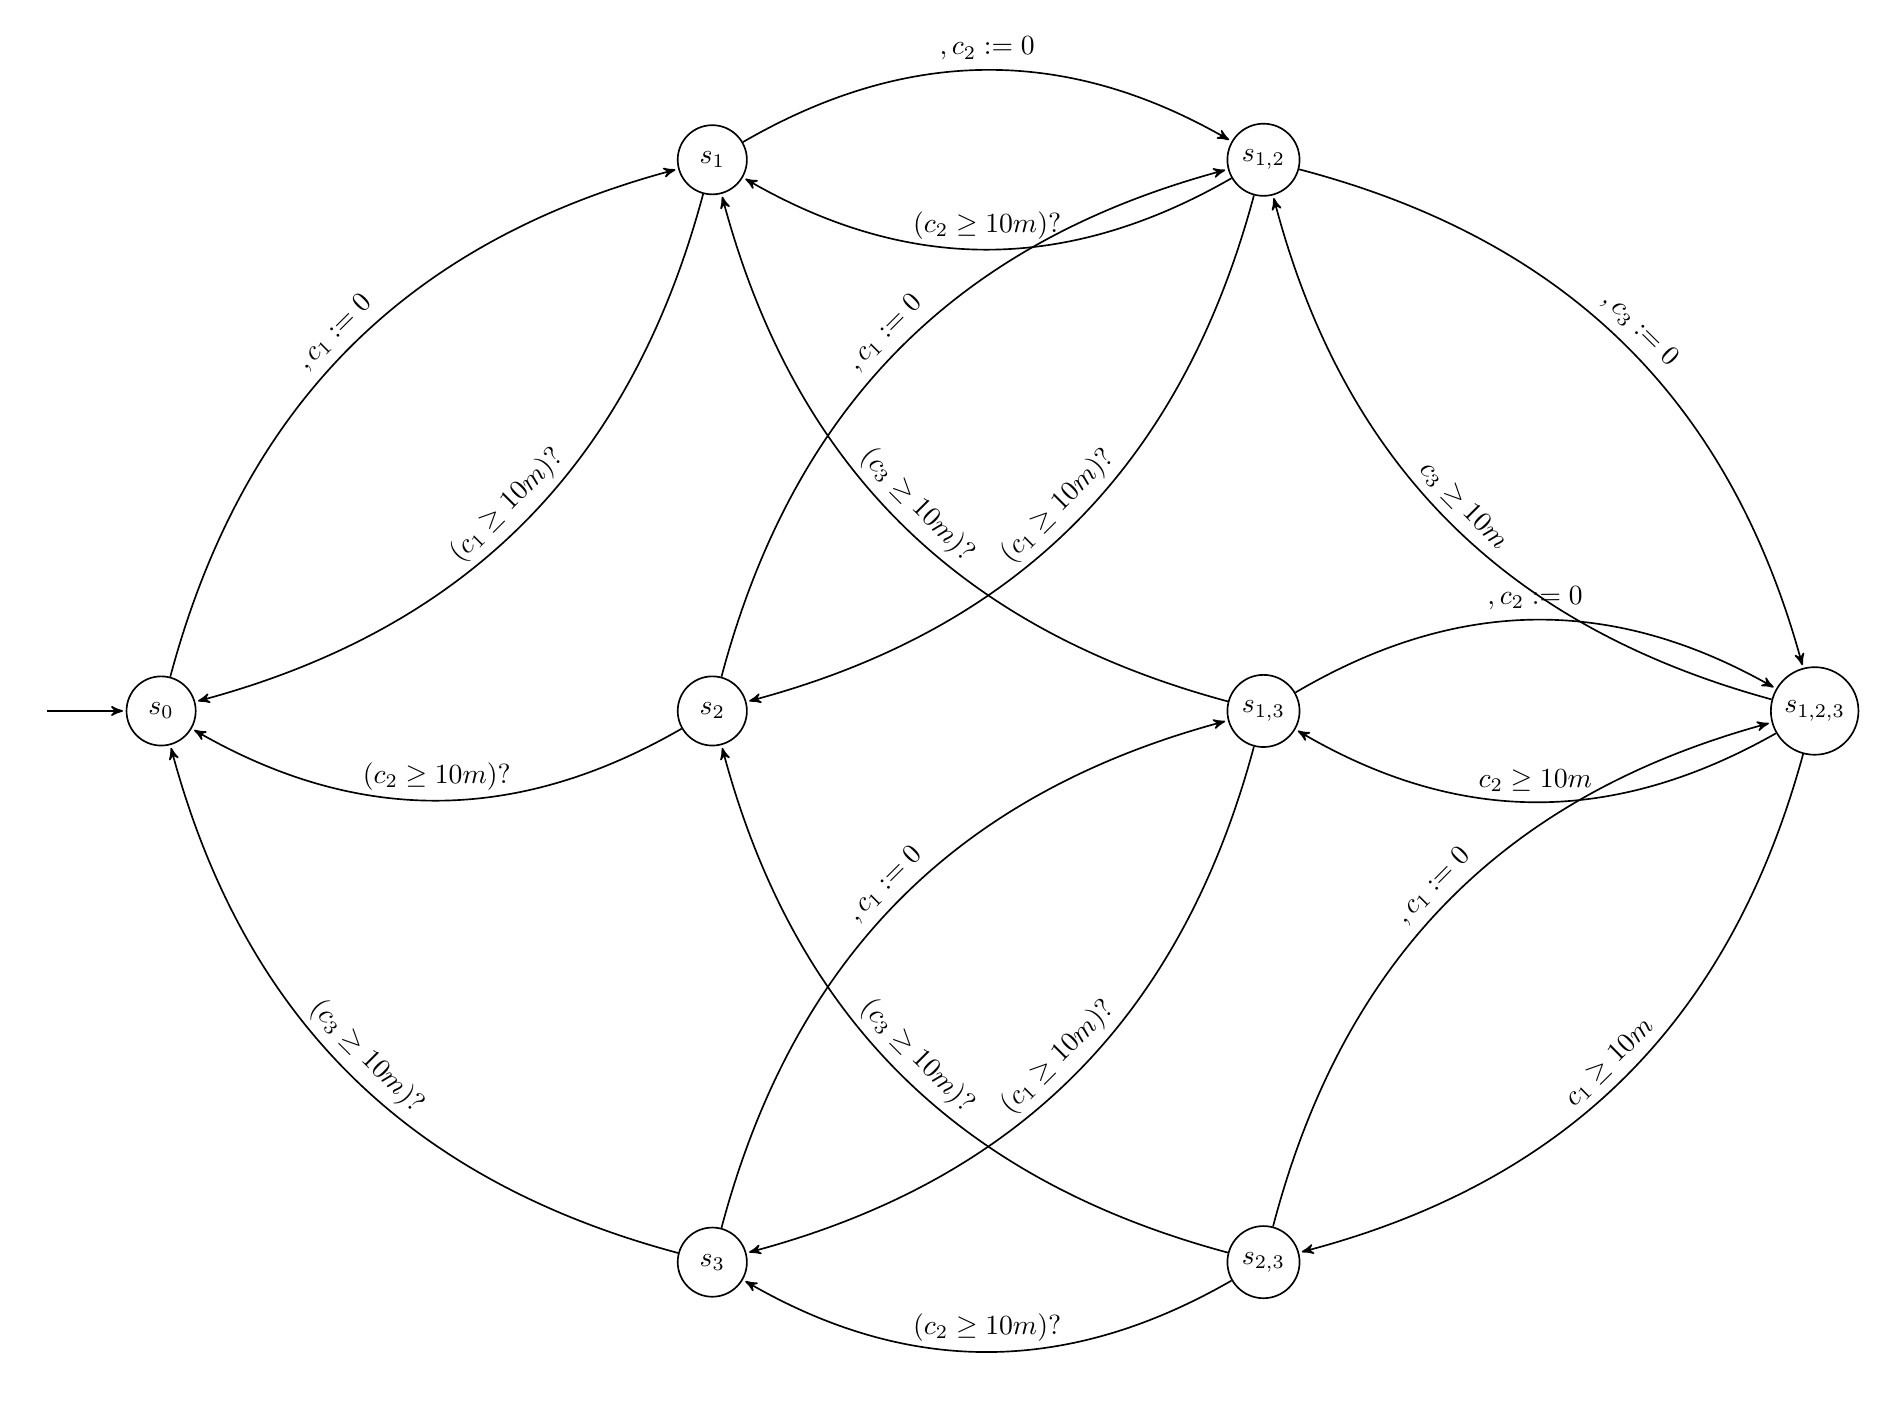
\begin{tikzpicture}[->,>=stealth',shorten >=1pt,auto,node distance=7cm, semithick]
	\node(start) {};
	\node[state] (S0) [right=0cm and 1cm of start]{$s_0$};
	\node[state] (S2) [right of=S0] {$s_2$};
	\node[state] (S1) [above of=S2] {$s_1$};
	\node[state] (S3) [below of=S2] {$s_3$};
	\node[state] (S12) [right of=S1] {$s_{1,2}$};
	\node[state] (S13) [below of=S12] {$s_{1,3}$};
	\node[state] (S23) [below of=S13] {$s_{2,3}$};
	\node[state] (S123) [right of=S13] {$s_{1,2,3}$};

	\path[every node/.style={sloped,anchor=south,auto=false}]
	 (start) edge node {} (S0)
	 (S1) edge [bend left] node {$(c_1 \geq 10m)?$} (S0)
	 (S2) edge [bend left] node {$(c_2 \geq 10m)?$} (S0)
	 (S3) edge [bend left] node {$(c_3 \geq 10m)?$} (S0)
	 (S0) edge [bend left] node {$\ccc, c_1 := 0$} (S1)
	 (S1) edge [bend left] node {$\ccc, c_2 := 0$} (S12)
	 (S12) edge [bend left] node {$(c_2 \geq 10m)?$} (S1)
	 (S13) edge [bend left] node {$(c_3 \geq 10m)?$} (S1)
	 (S2) edge [bend left] node {$\ccc, c_1 := 0$} (S12)
	 (S12) edge [bend left] node {$(c_1 \geq 10m)?$} (S2)
	 (S23) edge [bend left] node {$(c_3 \geq 10m)?$} (S2)
	 (S23) edge [bend left] node {$(c_2 \geq 10m)?$} (S3)
	 (S3) edge [bend left] node {$\ccc, c_1 := 0$} (S13)
	 (S13) edge [bend left] node {$(c_1 \geq 10m)?$} (S3)
	 (S12) edge [bend left] node {$\ccc, c_3 := 0$} (S123)
	 (S123) edge [bend left] node {$c_3 \geq 10m$} (S12)
	 (S13) edge [bend left] node {$\ccc, c_2 := 0$} (S123)
	 (S123) edge [bend left] node {$c_2 \geq 10m$} (S13)
	 (S23) edge [bend left] node {$\ccc, c_1 := 0$} (S123)
	 (S123) edge [bend left] node {$c_1 \geq 10m$} (S23);
\end{tikzpicture}
}
\end{frame}

\subsection{Generalization}
\begin{frame}
  \frametitle{1 Count}
  \centering

  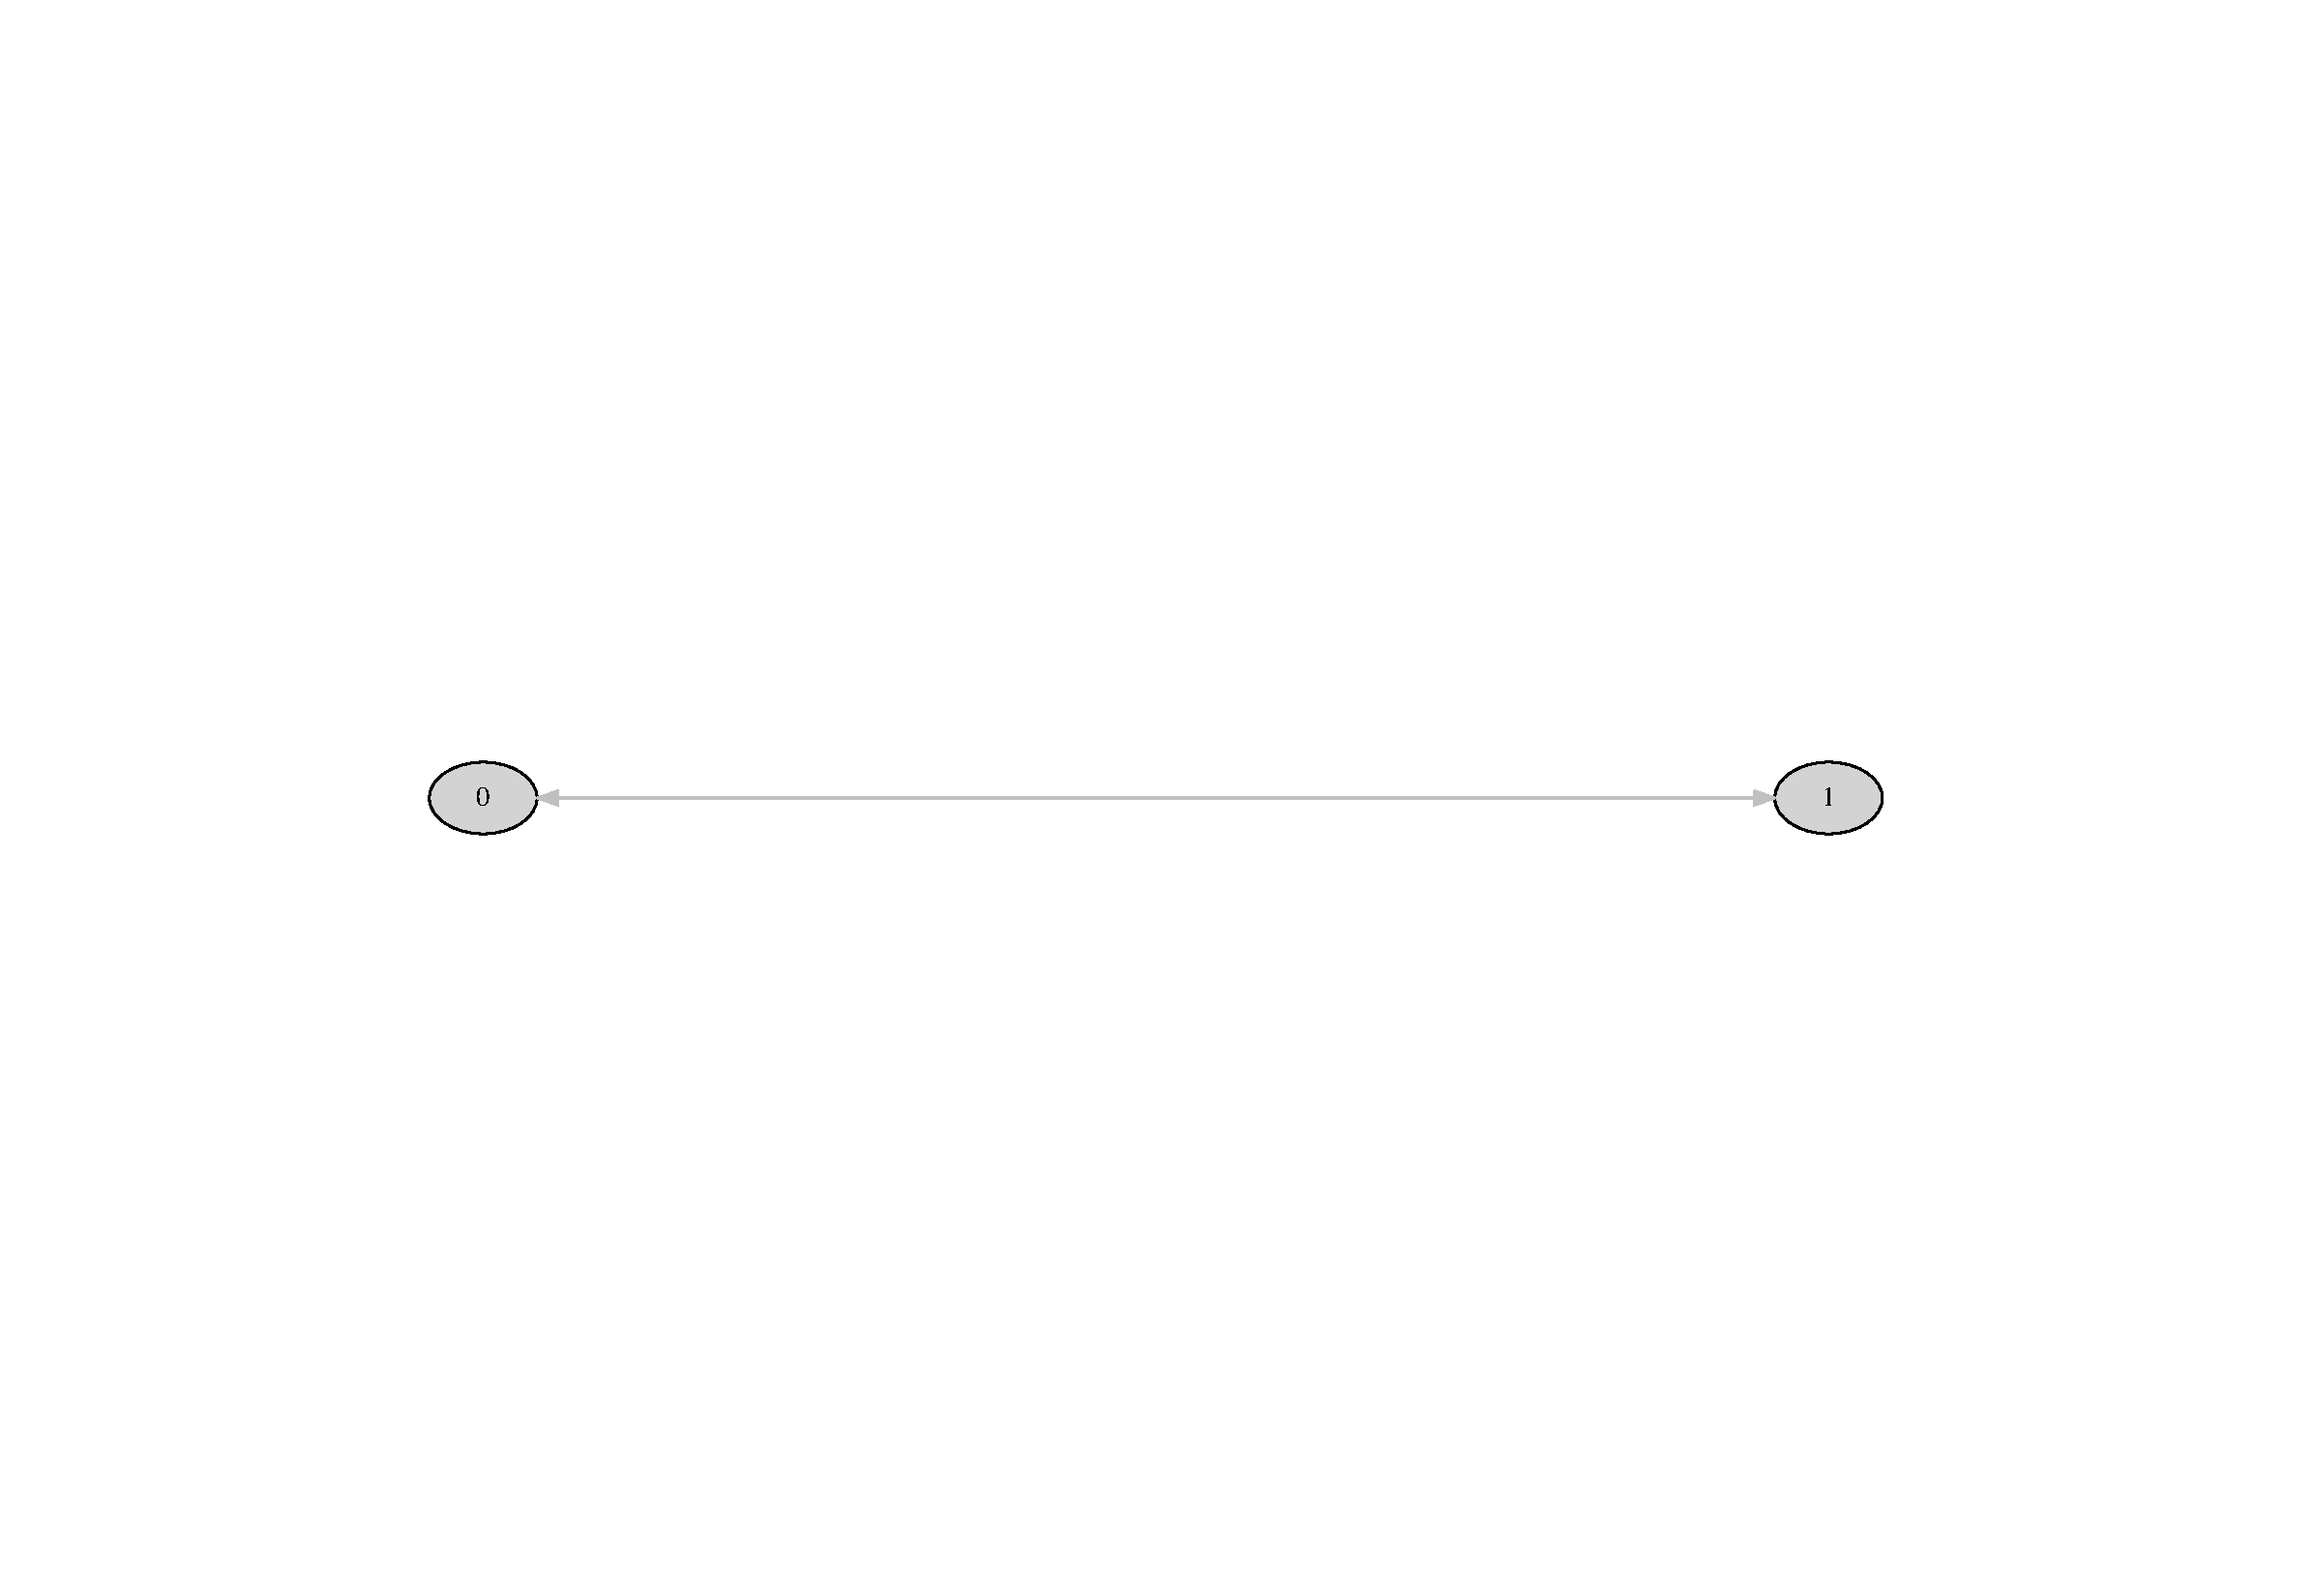
\includegraphics[width=\textwidth]{timed_automata/count1.pdf}
\end{frame}

\begin{frame}
  \frametitle{2 Count}
  \centering

  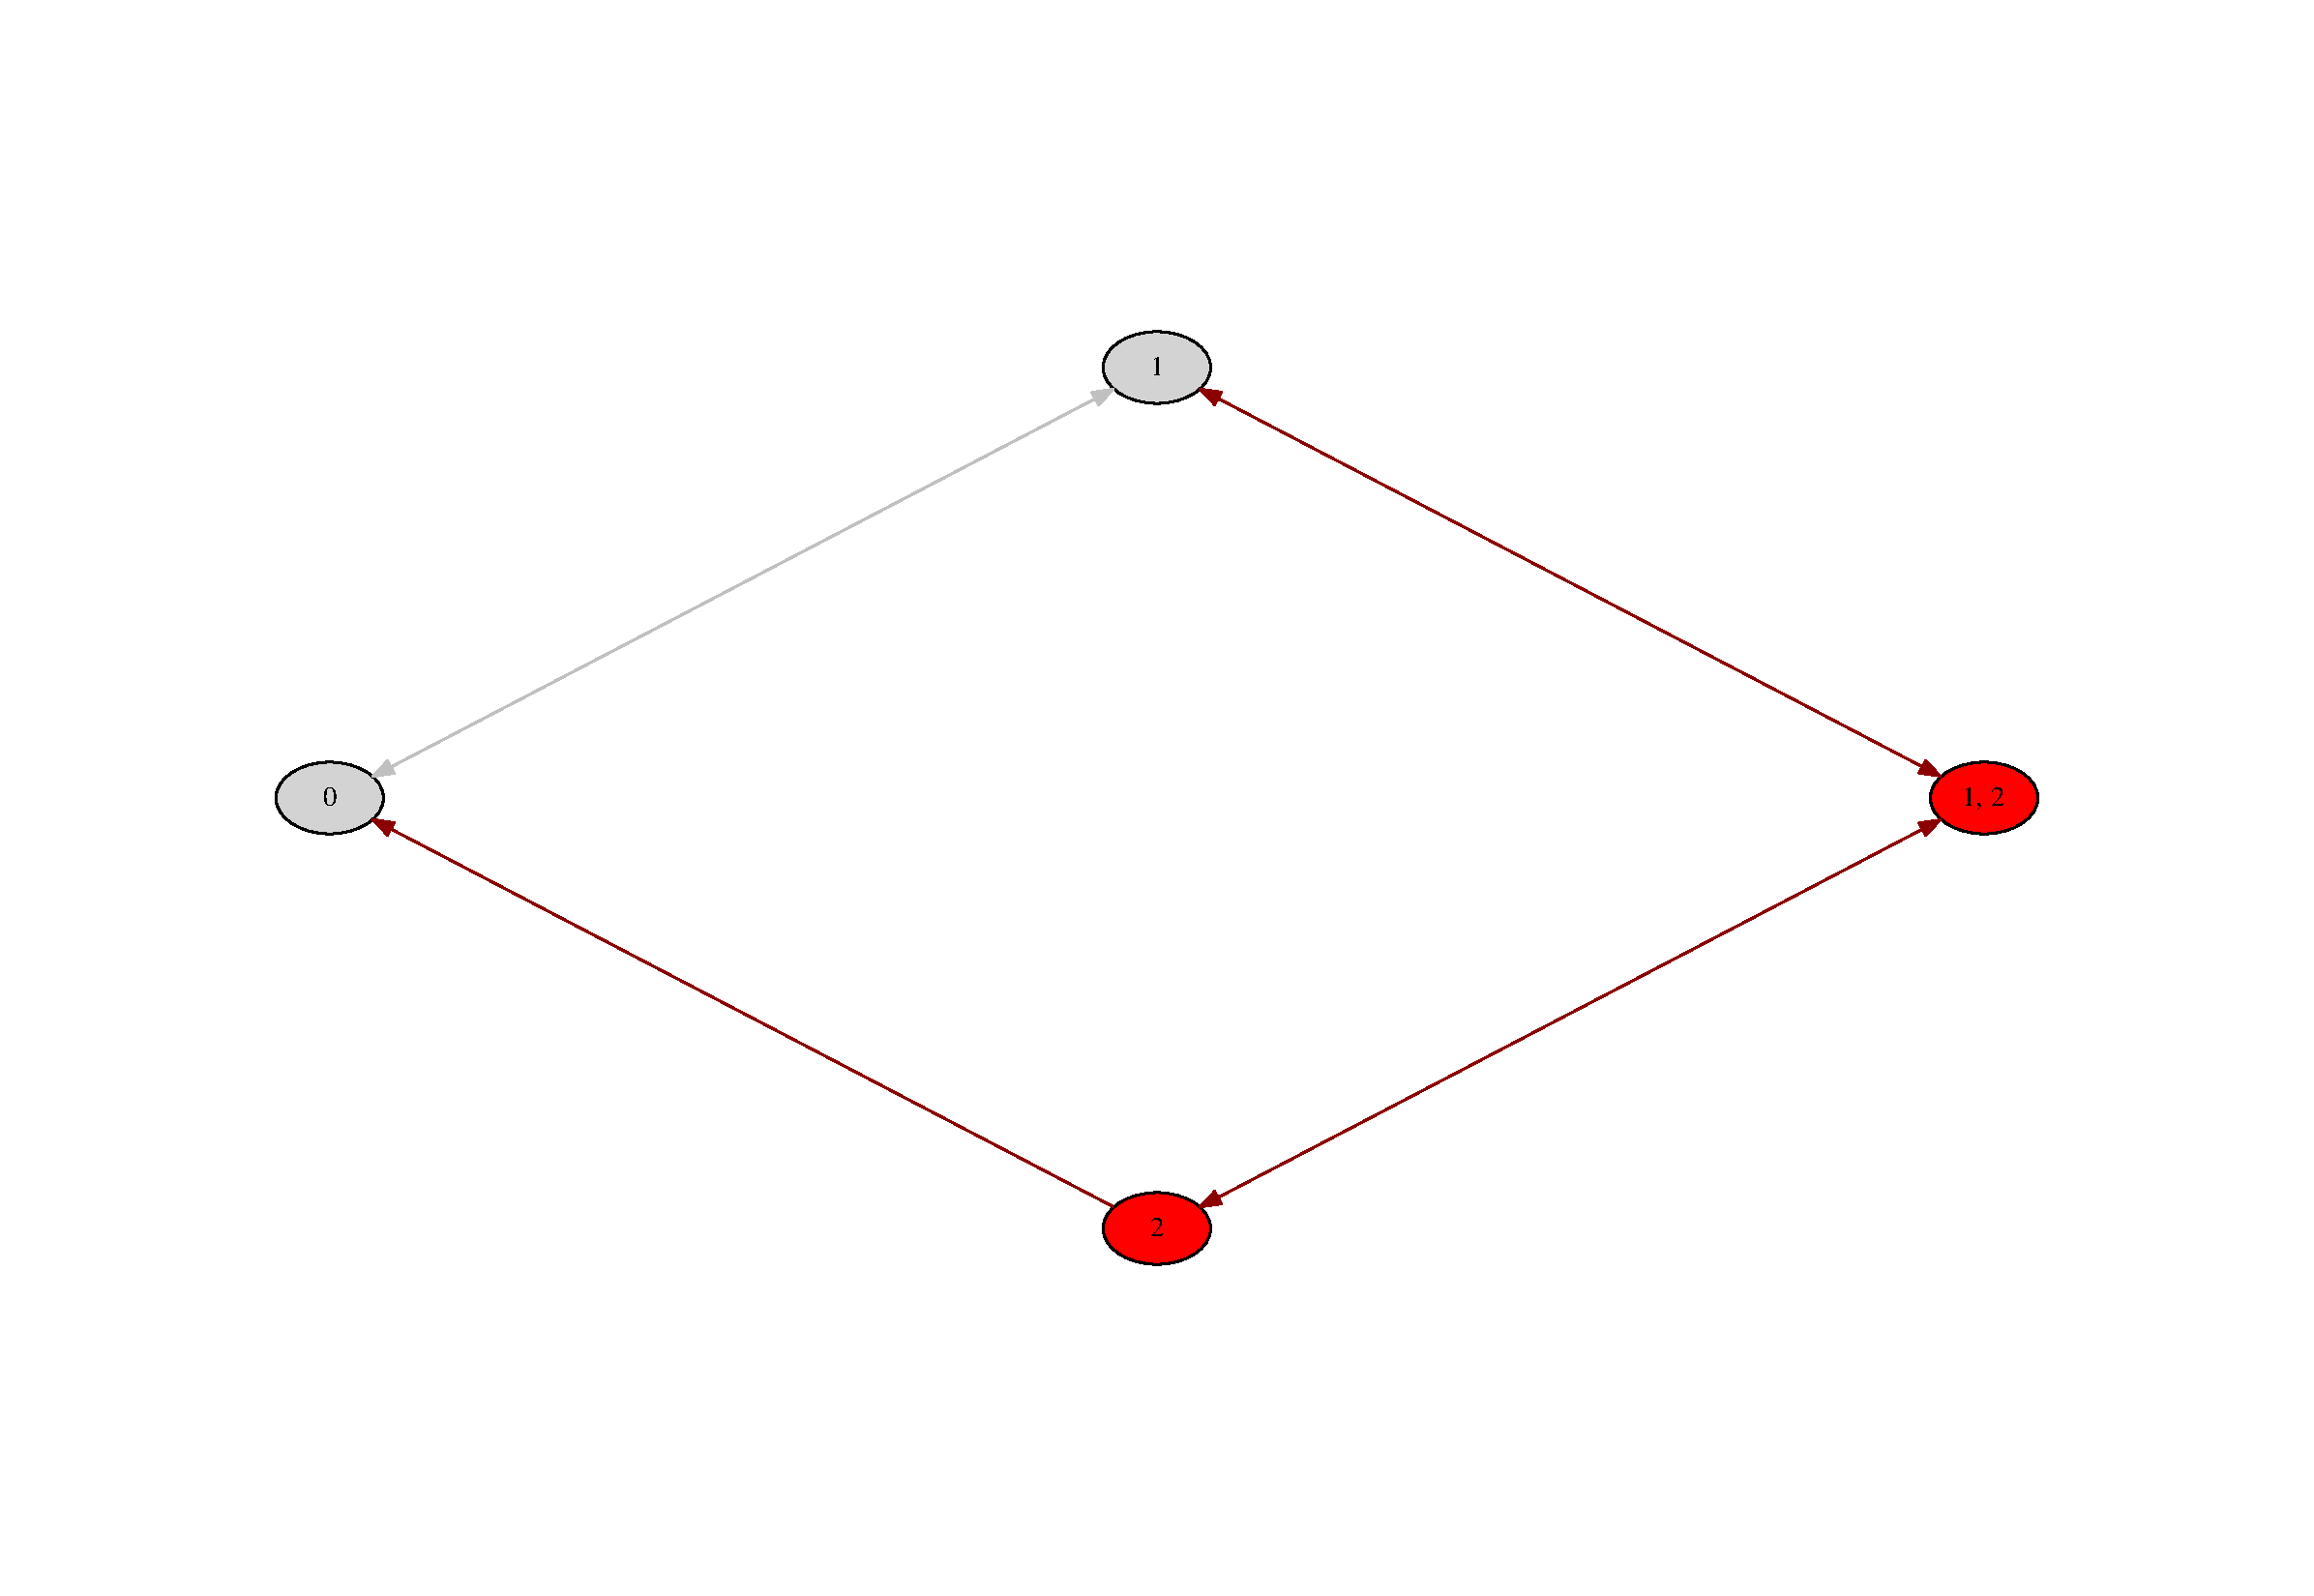
\includegraphics[width=\textwidth]{timed_automata/count2.pdf}
\end{frame}

\begin{frame}
  \frametitle{3 Count}
  \centering

  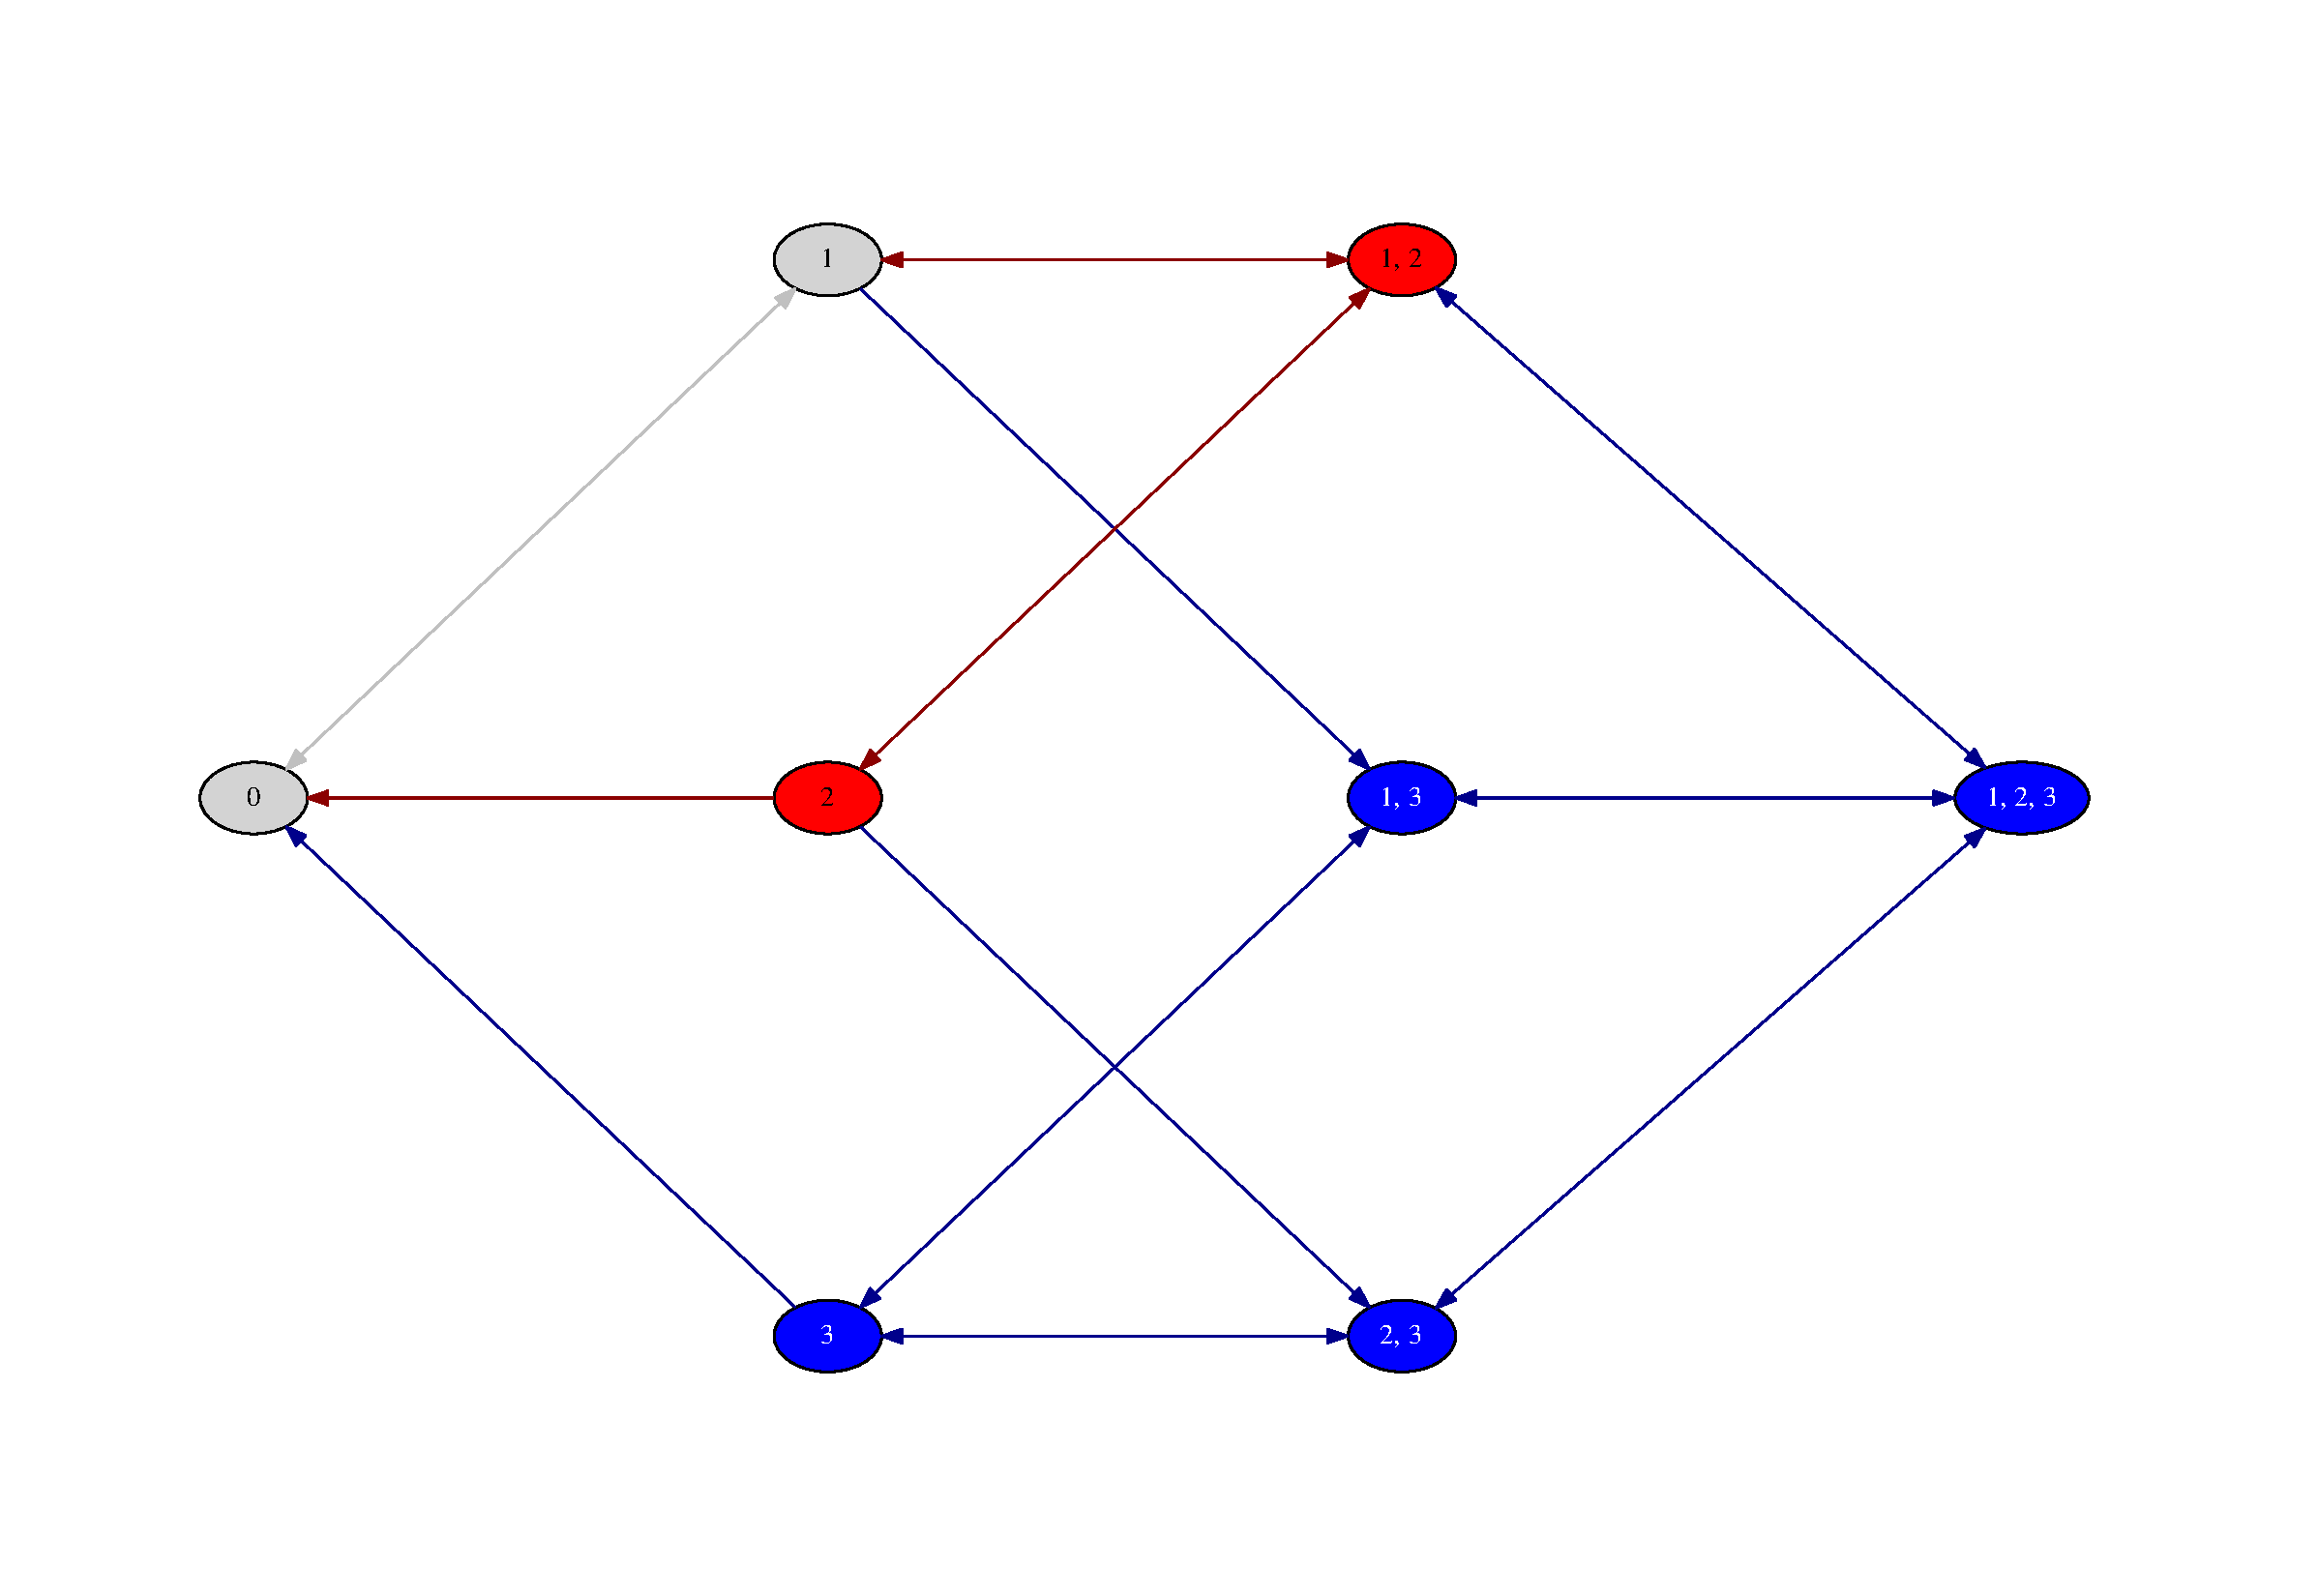
\includegraphics[width=\textwidth]{timed_automata/count3.pdf}
\end{frame}

\begin{frame}
  \frametitle{4 Count}
  \centering

  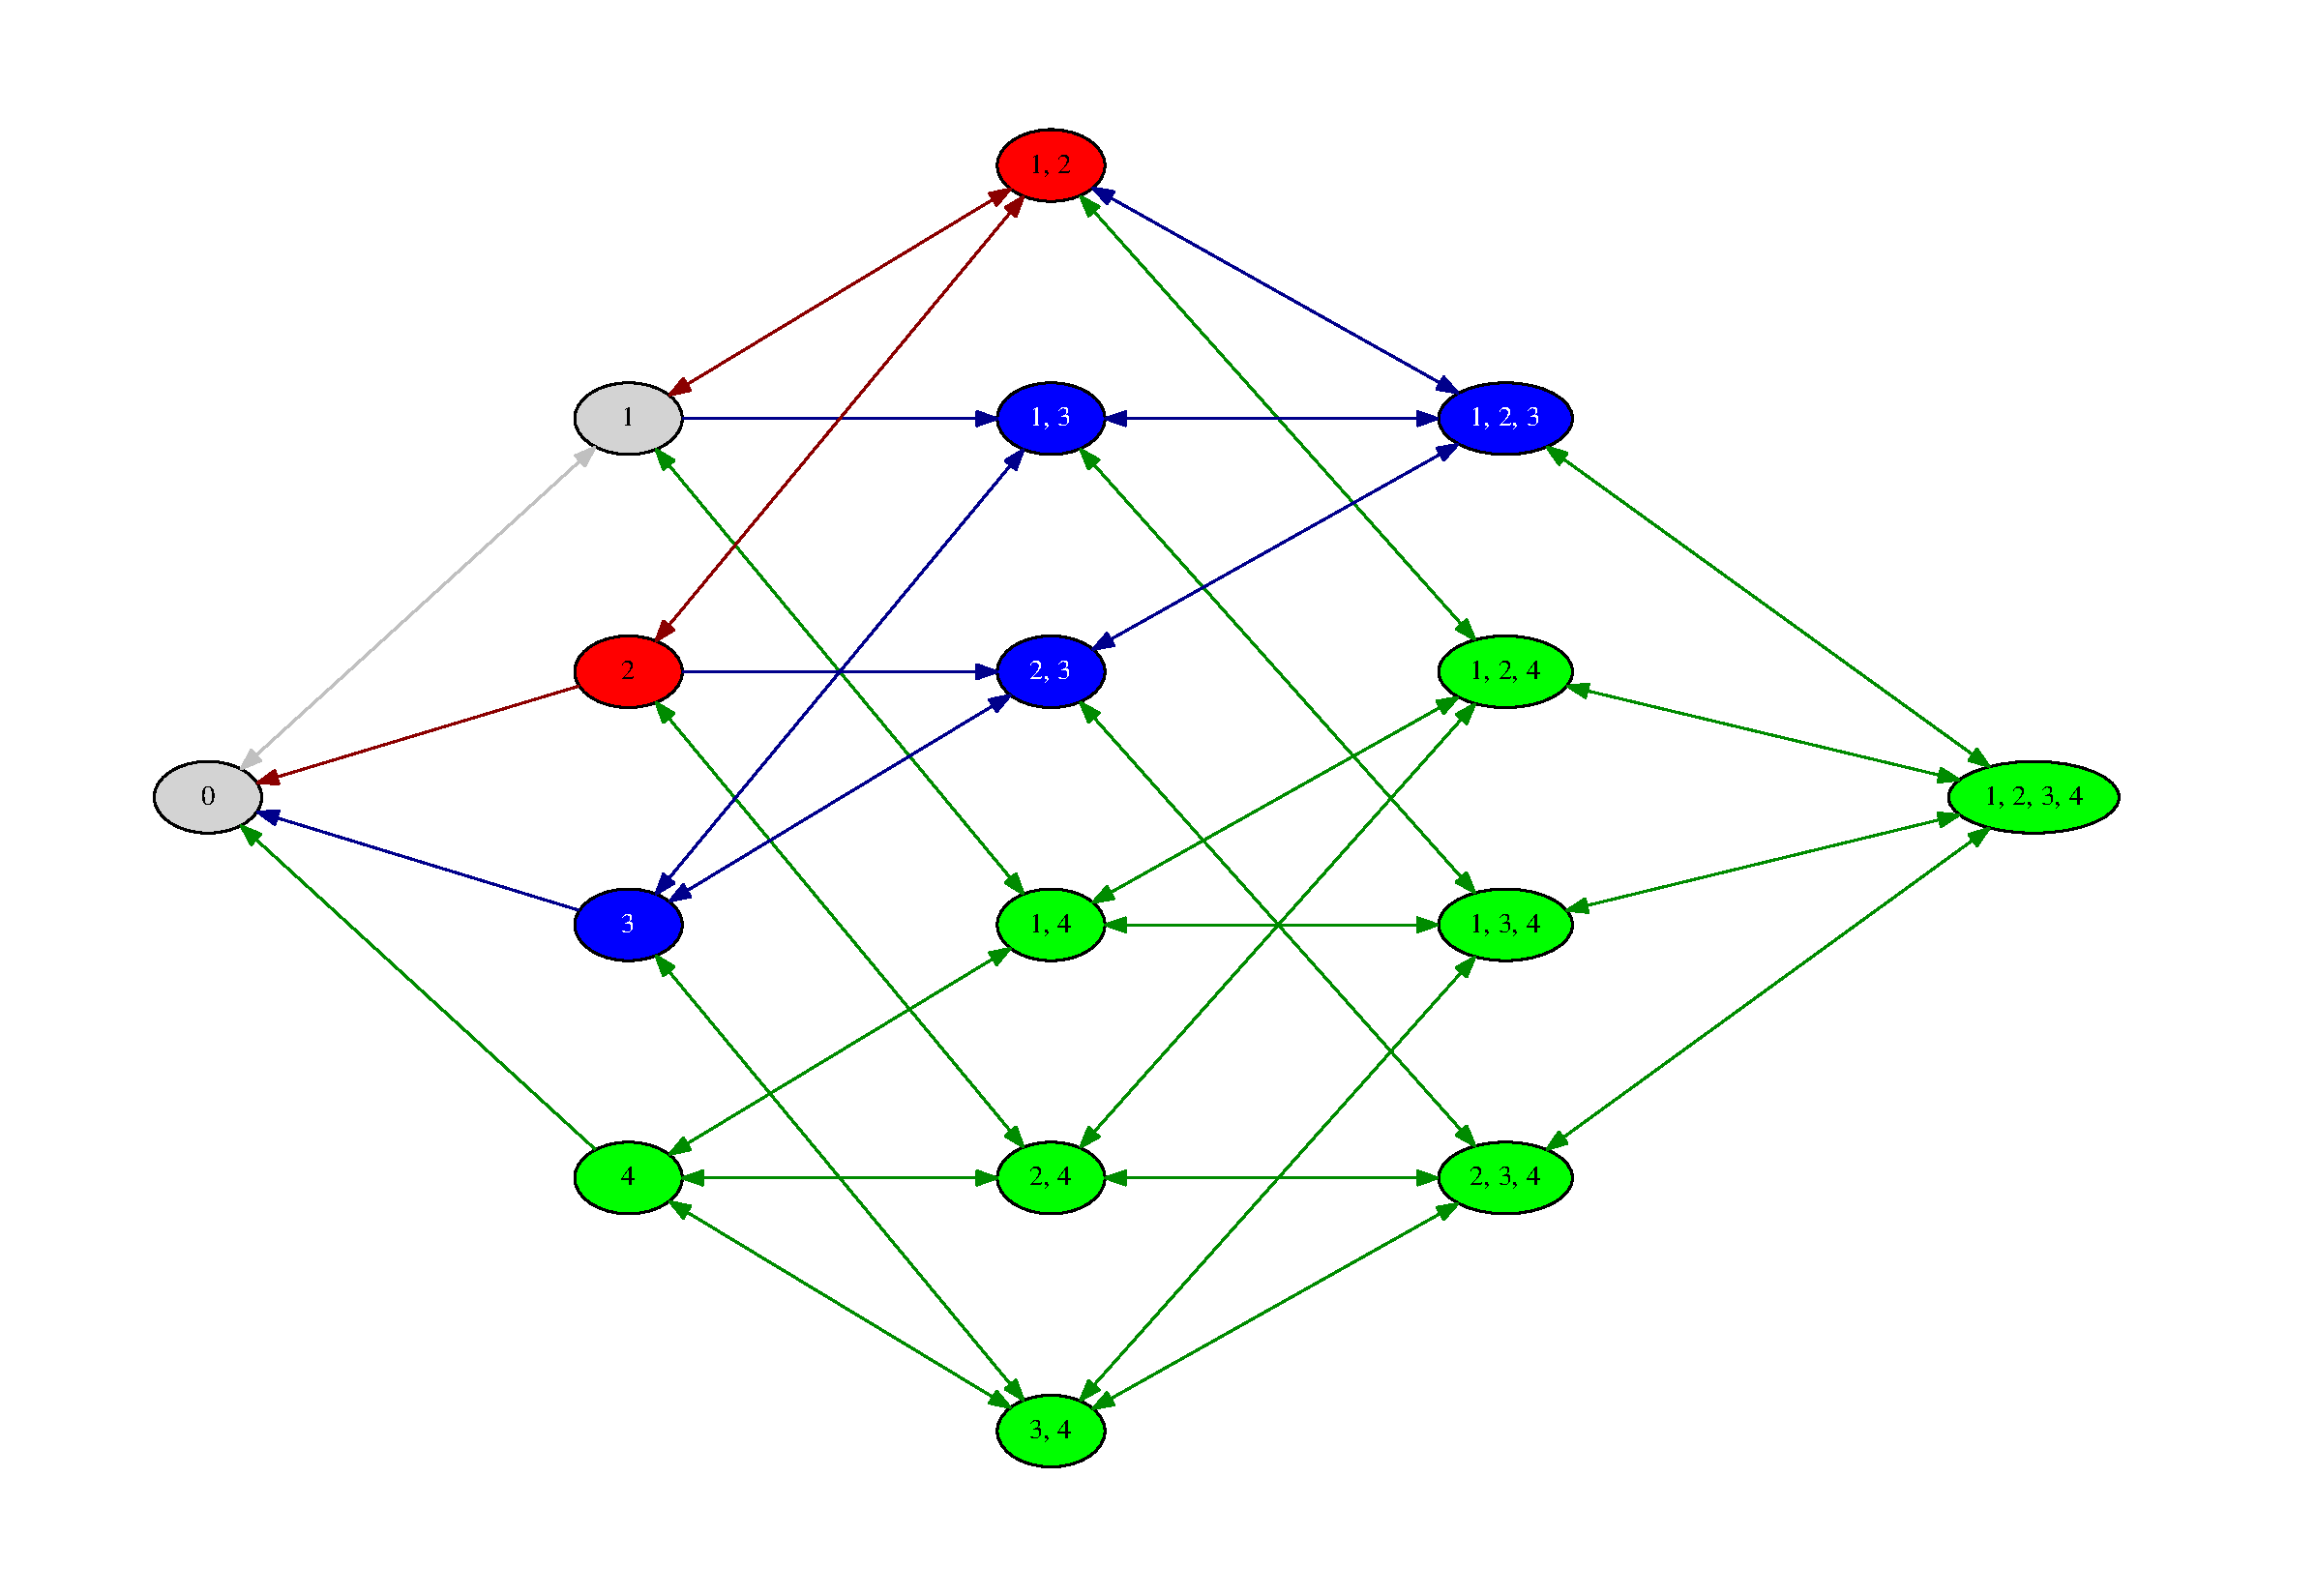
\includegraphics[width=\textwidth]{timed_automata/count4.pdf}
\end{frame}

\subsection{Implementation}
\begin{frame}
  \frametitle{Implementation}

  \begin{itemize}
    \item Array for count
  \end{itemize}
\end{frame}

{\aauwavesbg
\begin{frame}[plain,noframenumbering]
  \finalpage{The end!}
\end{frame}}
%%%%%%%%%%%%%%%%

\end{document}
